\section*{Results and Analysis}
\label{Results}
%
Using a 2-way ANOVA, a significant assessor effect (p<0.01) has been found on the "Dark - Light" attribute, which means that the assessors disagree about how light/dark the speakers are. See \autoref{fig:AssessorEffect}. This could mean that people do not have the same understanding of what it means for something to be light or dark.
%
\begin{figure}[H]
\centering
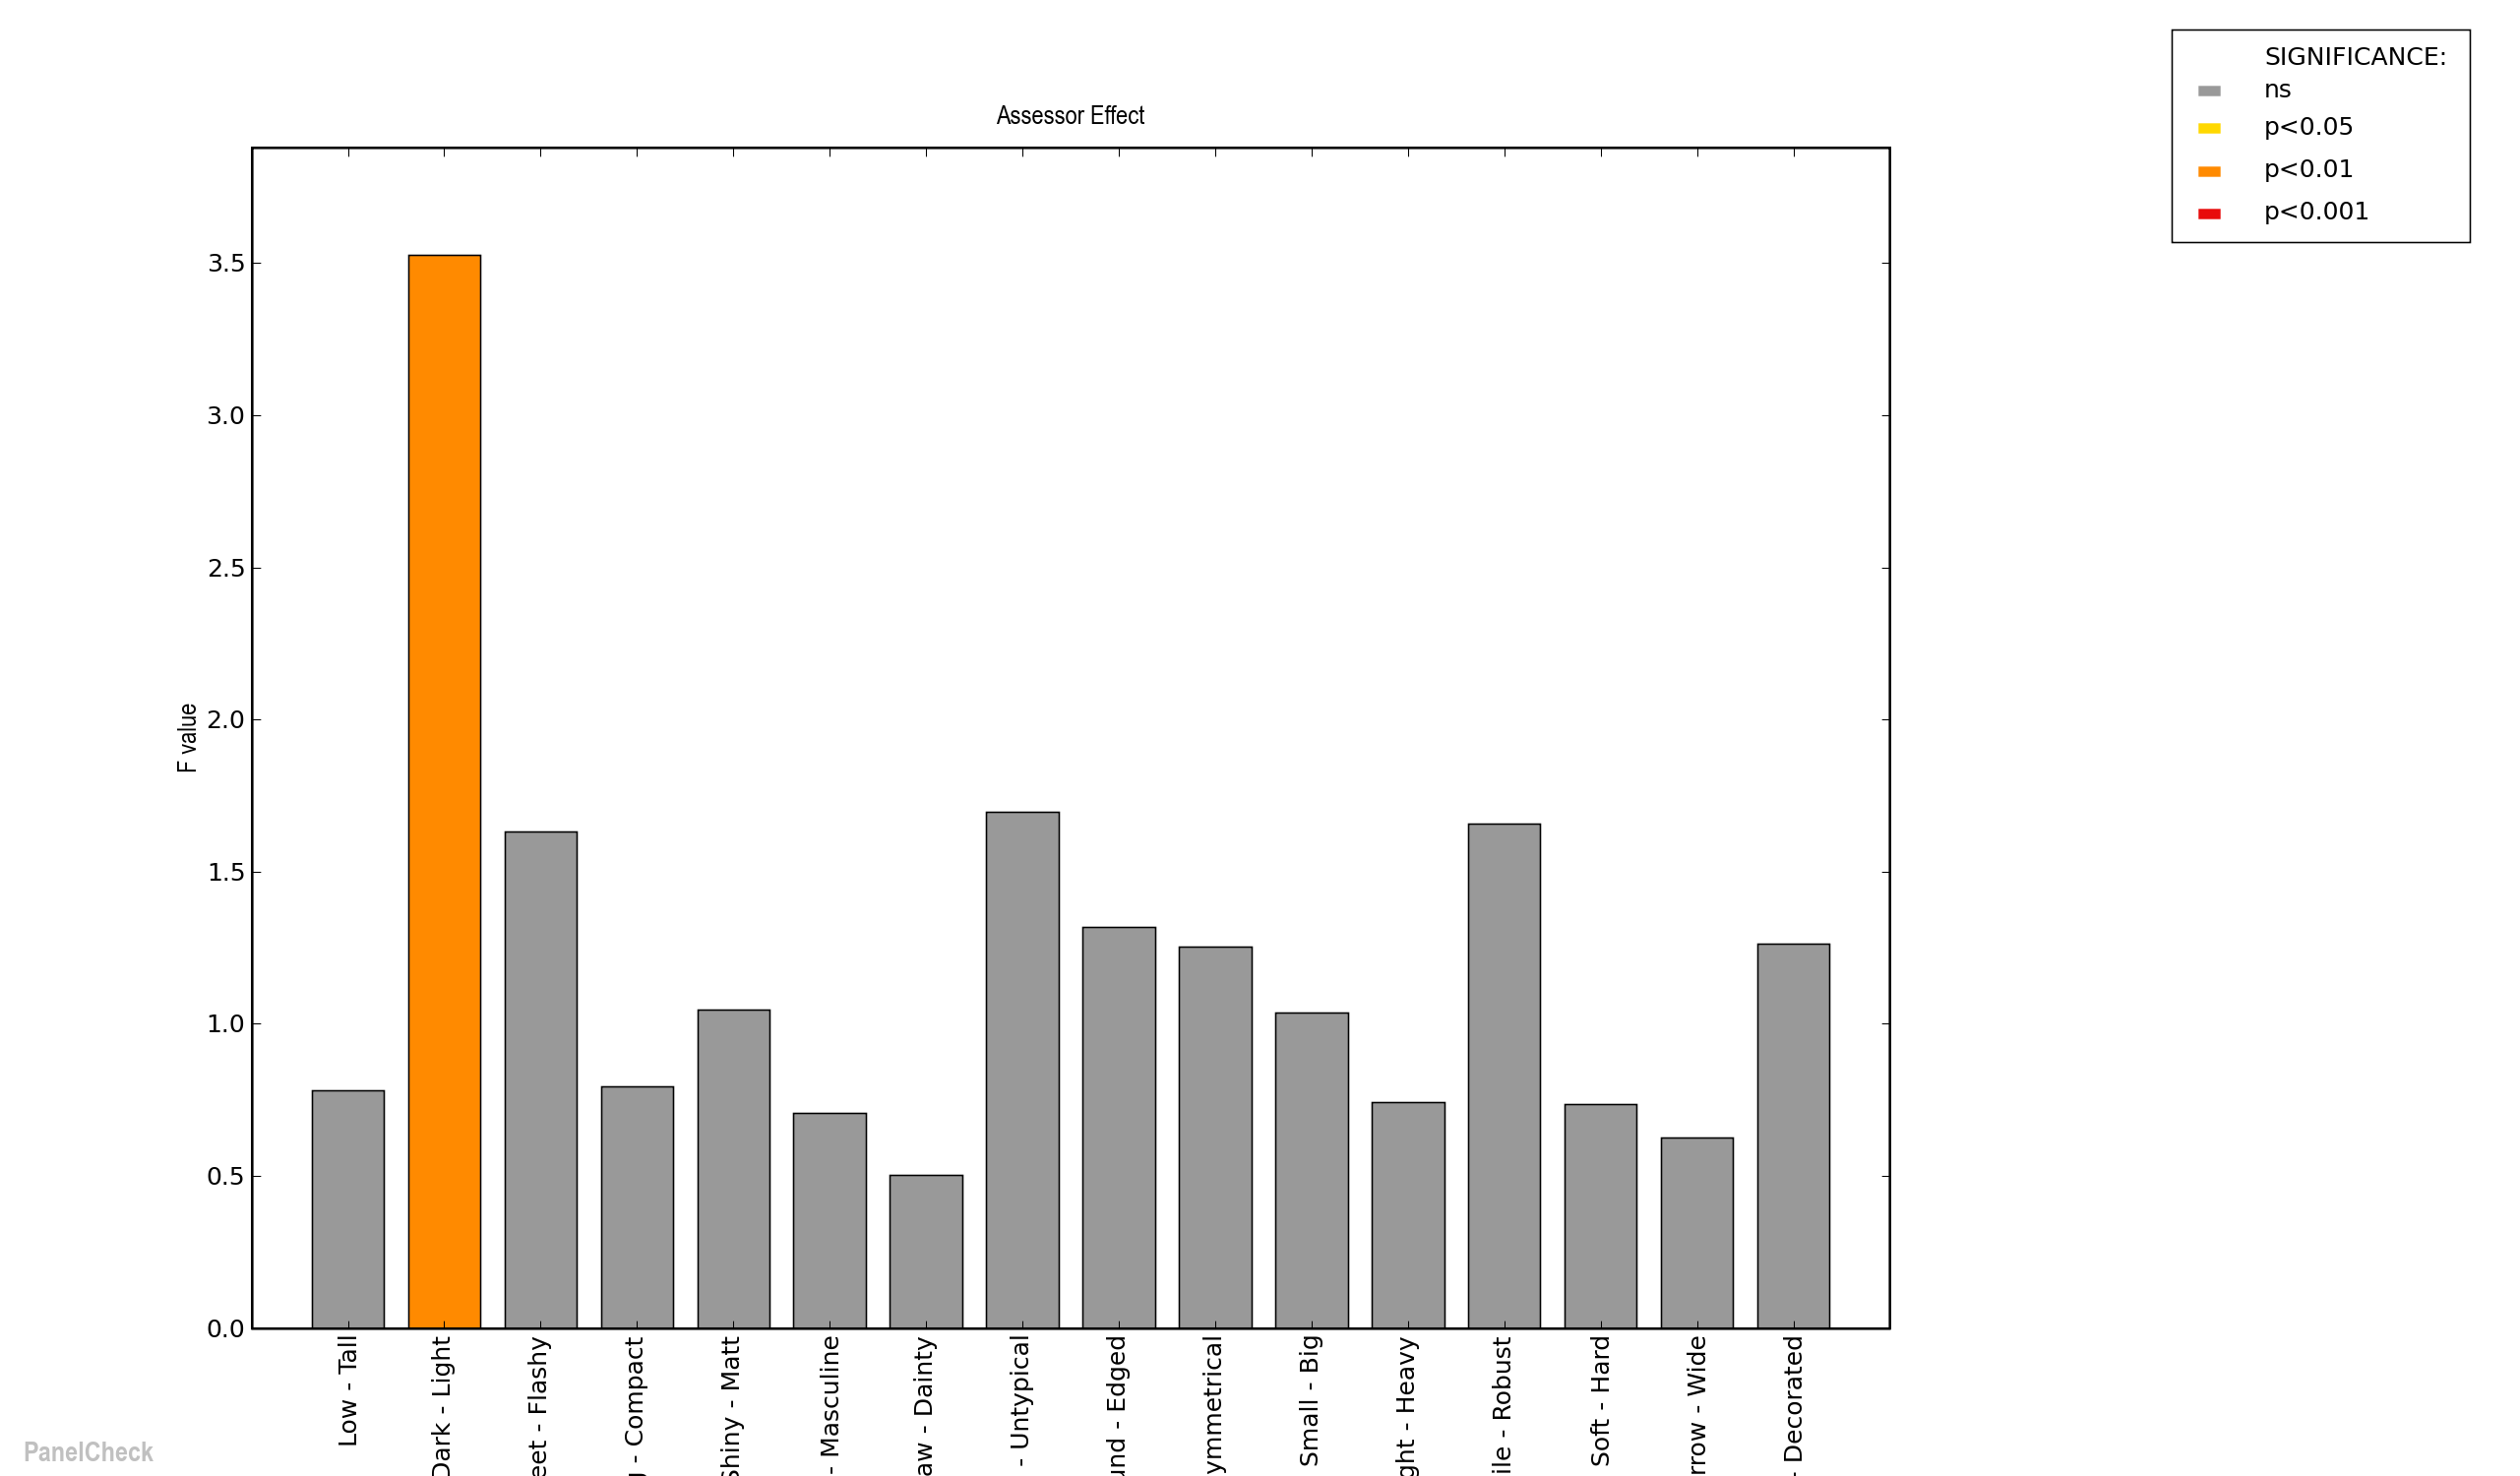
\includegraphics[width =0.9\textwidth]{Figure/AssessorEffect.png} 
\caption{A plot showing the assessor effect. The variance was only significantly different in the results relating to the "Dark - Light" attribute, indicated by the orange bar. This means that the assessors did not agree upon which of the speakers were the lightest or darkest.}
\label{fig:AssessorEffect}
\end{figure}
\noindent
%
Regarding the product effect on ratings, all attributes are rated significantly different at at least p<0.01, except for "Symmetrical - Asymmetrical". That means that the speaker model has an influence on the ratings of all the attributes, except for symmetry, which is unaffected of which speaker model is rated.
%
\begin{figure}[H]
\centering
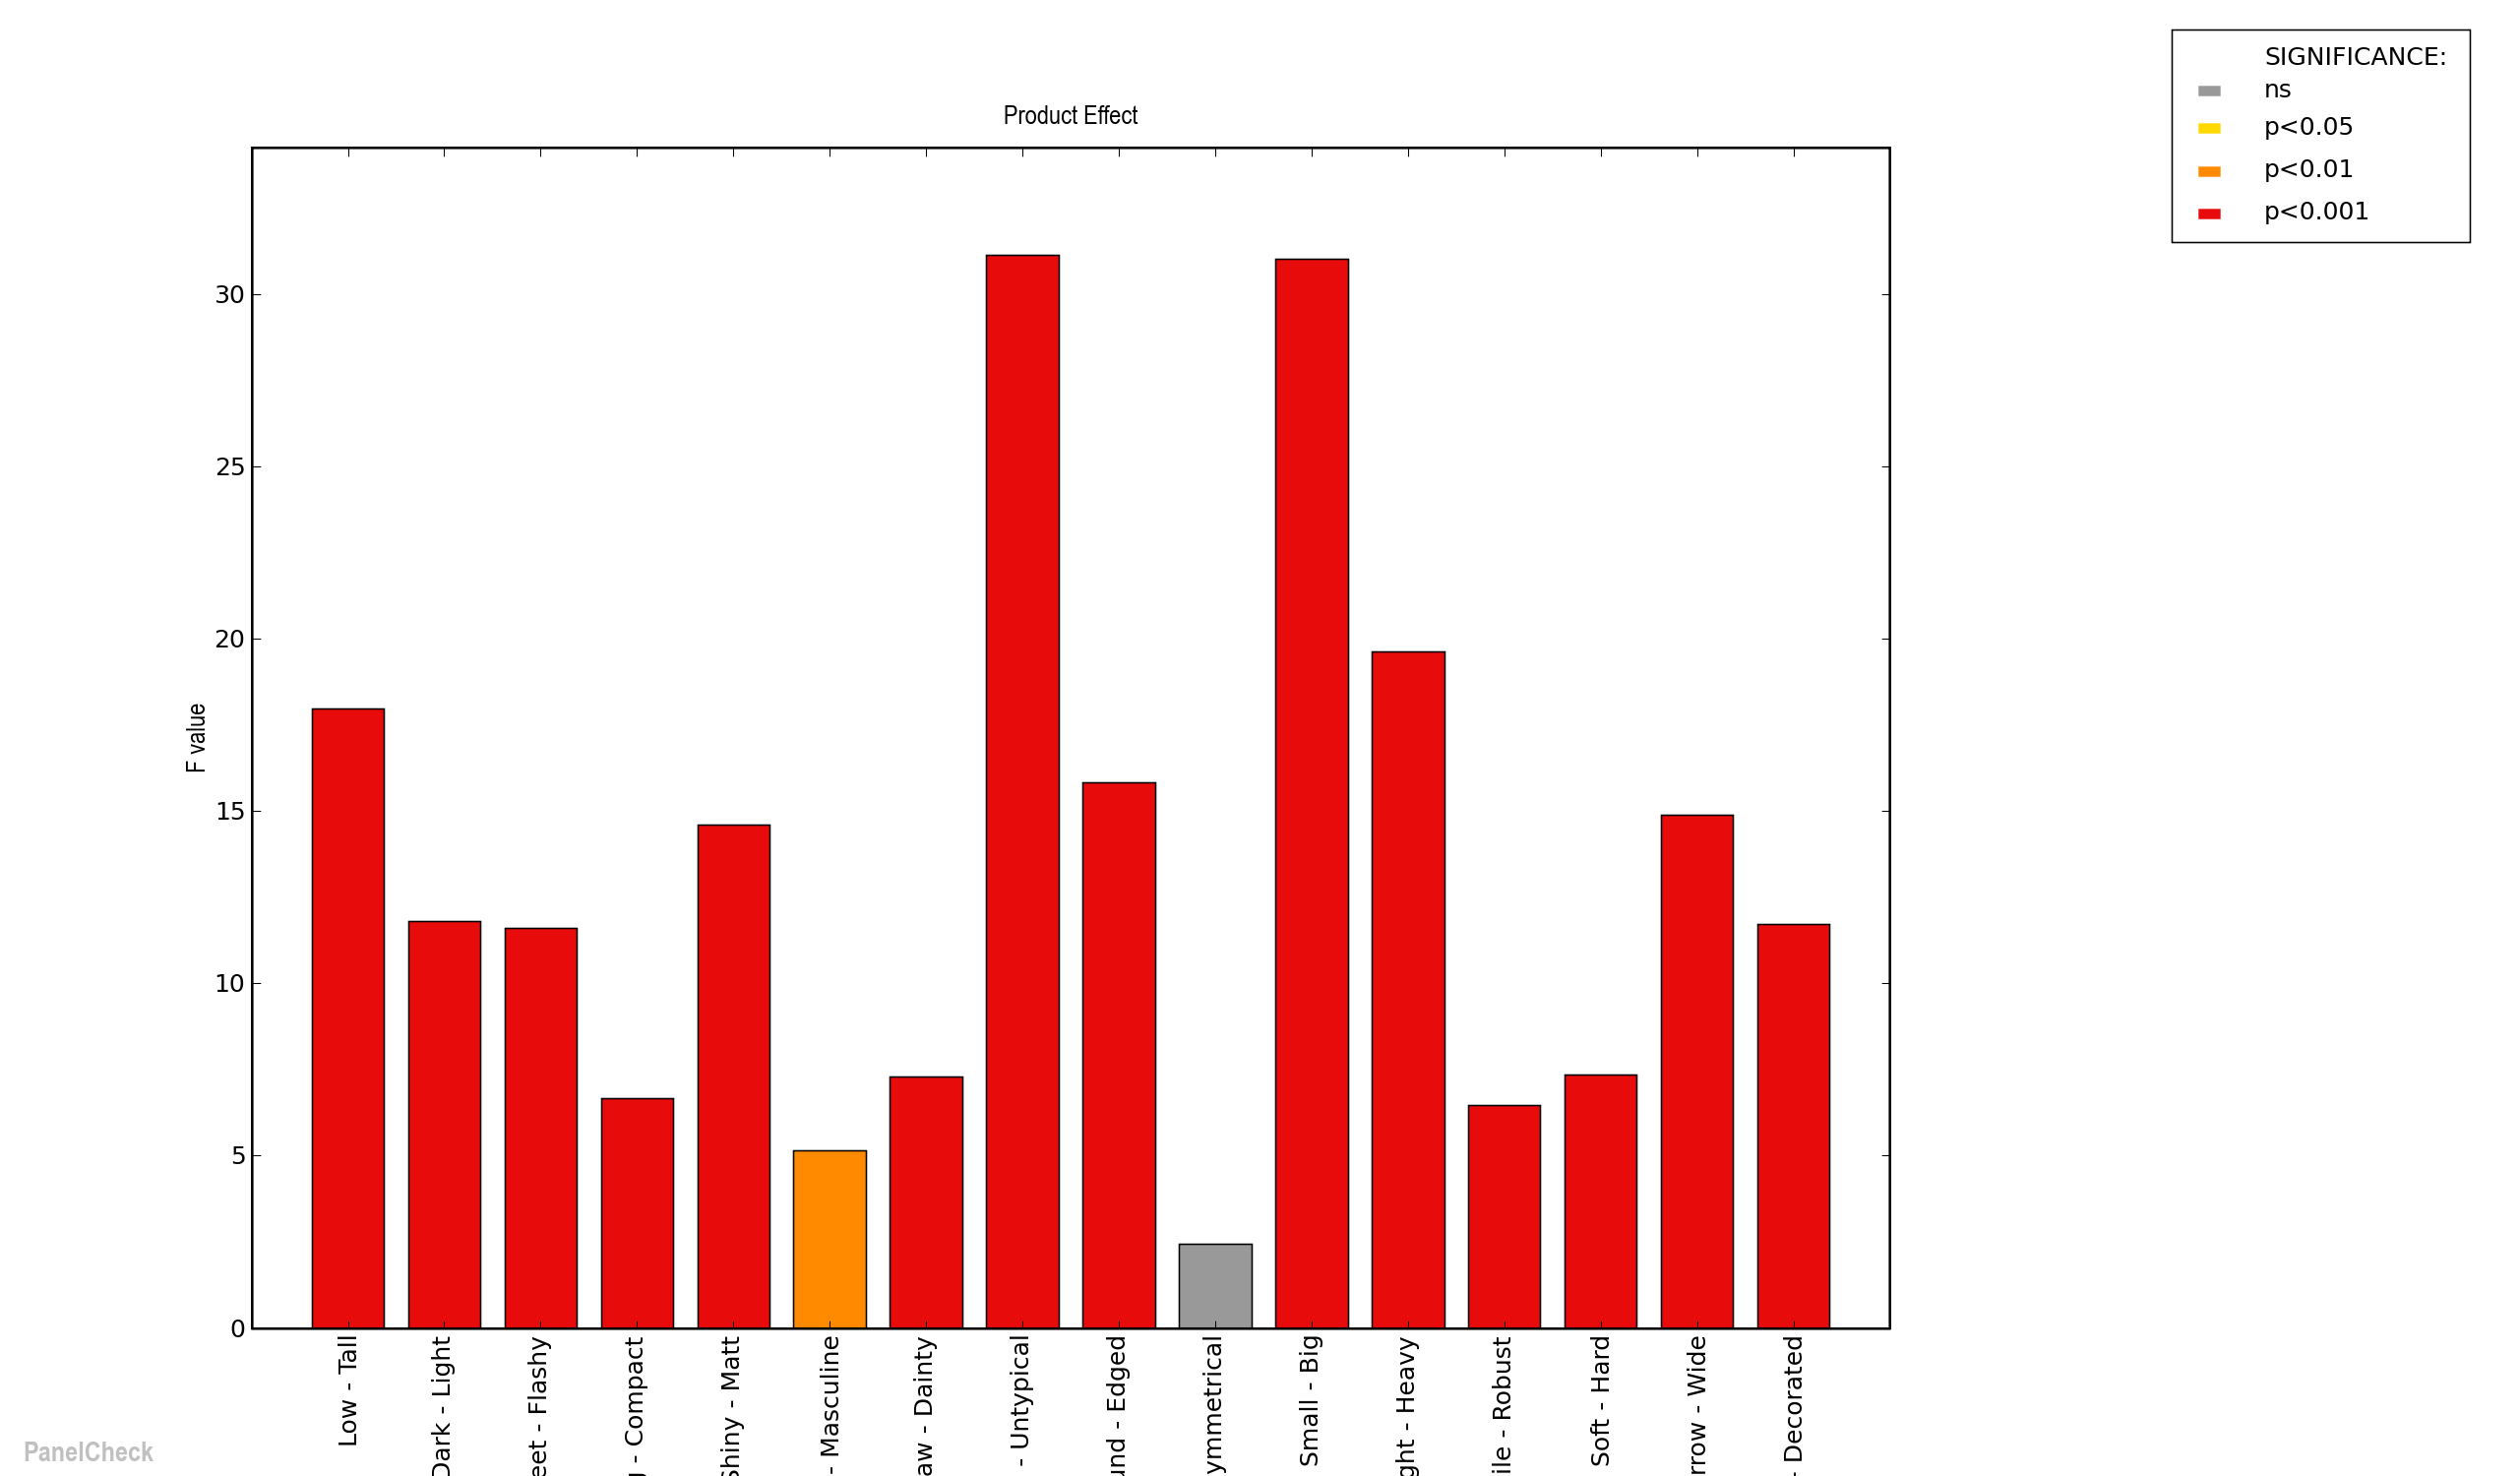
\includegraphics[width = 0.9\textwidth]{Figure/ProductEffect.png} 
\caption{A plot showing the product effect. The only attribute which is unaffected by speaker model is the one regarding symmetry, indicated by the grey bar. All other attributes are affected by speaker model, indicated by the red bars for p<0.001 and orange bar for p<0.01.}
\label{fig:ProductEffect}
\end{figure}
\newpage
\noindent
%
This can be confirmed by looking at the means and standard deviations for the different attributes. For example, in \autoref{fig:AttributeImportance}, the symmetry attribute has a very little standard deviation, which means that it is fairly unaffected by speaker model, compared to some of the other attributes. This means that the attribute is unimportant for the rating of the speakers.
%
\begin{figure}[H]
\centering
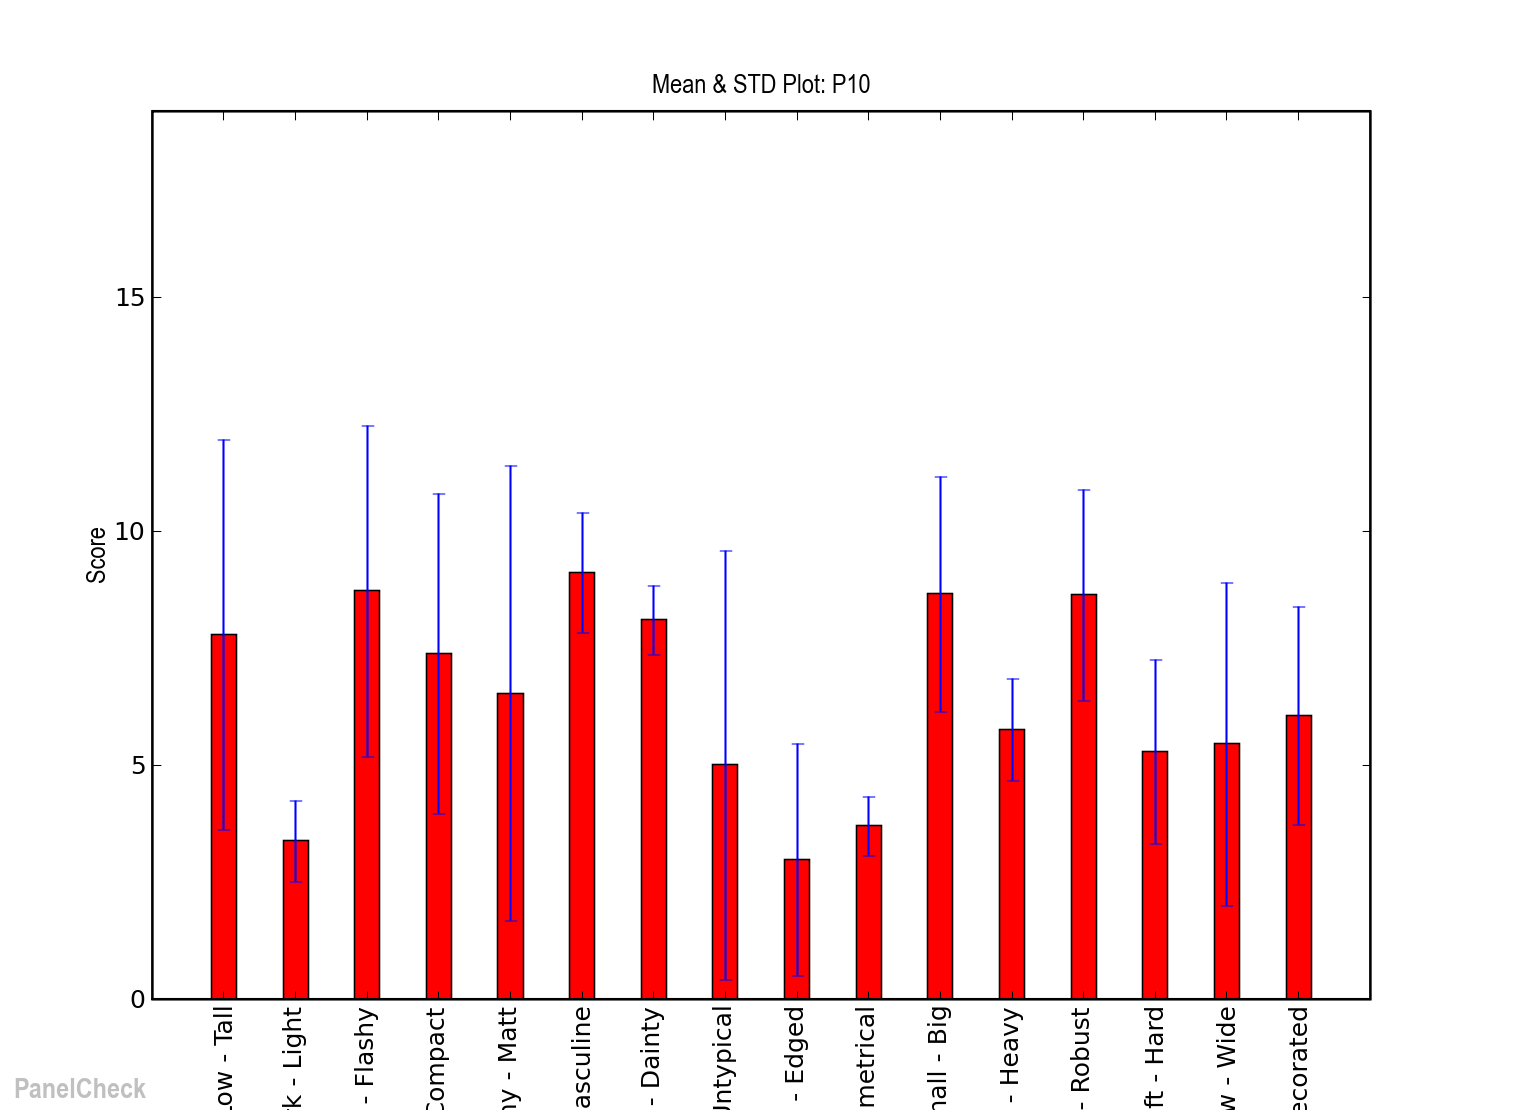
\includegraphics[width =0.9\textwidth]{Figure/AttributeImportance.png} 
\caption{A plot showing attribute importance according to their individual mean and standard deviation.}
\label{fig:AttributeImportance}
\end{figure}
\newpage
\noindent
%
Looking at the product effect alone for all of the five speakers does not tell us anything about which of the speakers where rated different than the others, but only that some of them were. By doing a 2-way ANOVA on only two of the speakers, it is possible to see which attributes separates the two. For example, when comparing the Beolab 4000 with the Beolab 6000 (see \autoref{fig:speakers}), the main differentiators are: \textit{Low - Tall}, \textit{Light - Dark}, and \textit{Wide - Narrow}, as shown in \autoref{fig:4000vs6000}. This approach can be repeated across the different combinations of speakers, to assess how each differs from the others.
%
\begin{figure}[H]
\centering
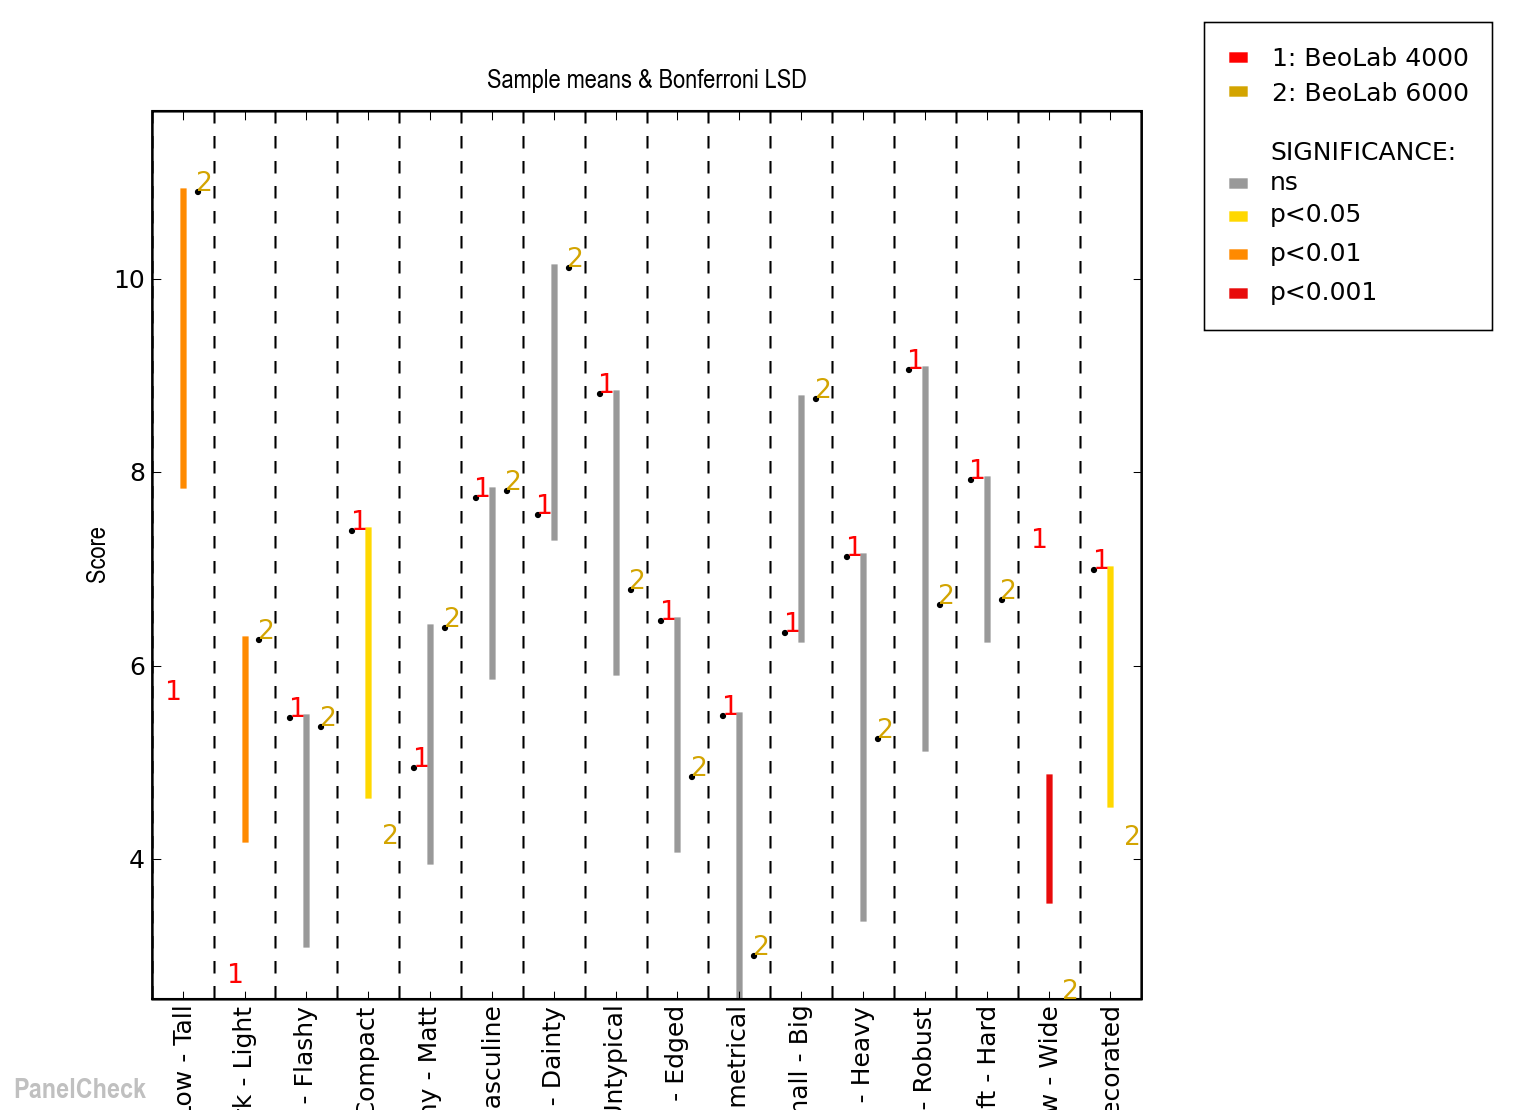
\includegraphics[width = 0.9\textwidth]{Figure/4000vs6000.png} 
\caption{Comparison of the attribute ratings for the Beolab 4000 and the Beolab 6000. It is possible to see which of the attributes are significantly different from each other. In this example it is: "Low - Tall", "Light - Dark", and "Wide - Narrow".}
\label{fig:4000vs6000}
\end{figure}
\newpage
\noindent
%
It is possible to look at a spider plot in order to get a sense of how the speakers were rated overall, as illustrated on \autoref{fig:spider_plot}. Here the left word is the inner point and the right word is the outer point. For example the BeoLab 5 overall scores the highest in the attributes: \textit{Flashy}, \textit{Decorated}, \textit{Wide}, and \textit{Untypical}. This seems reasonable when presented with the speakers next to each other in \autoref{fig:speakers}. In general this paints a fitting picture regarding which features stand out the most and it creates a unique attribute profile for each speaker when shown individually. Though when shown all together as in \autoref{fig:spider_plot} some points risk ending up on top of each other and some insights may be lost due to this. That being said, a spider plot is generally considered quite useful in displaying multivariate data visually. 
%
\begin{figure}[H]
\centering
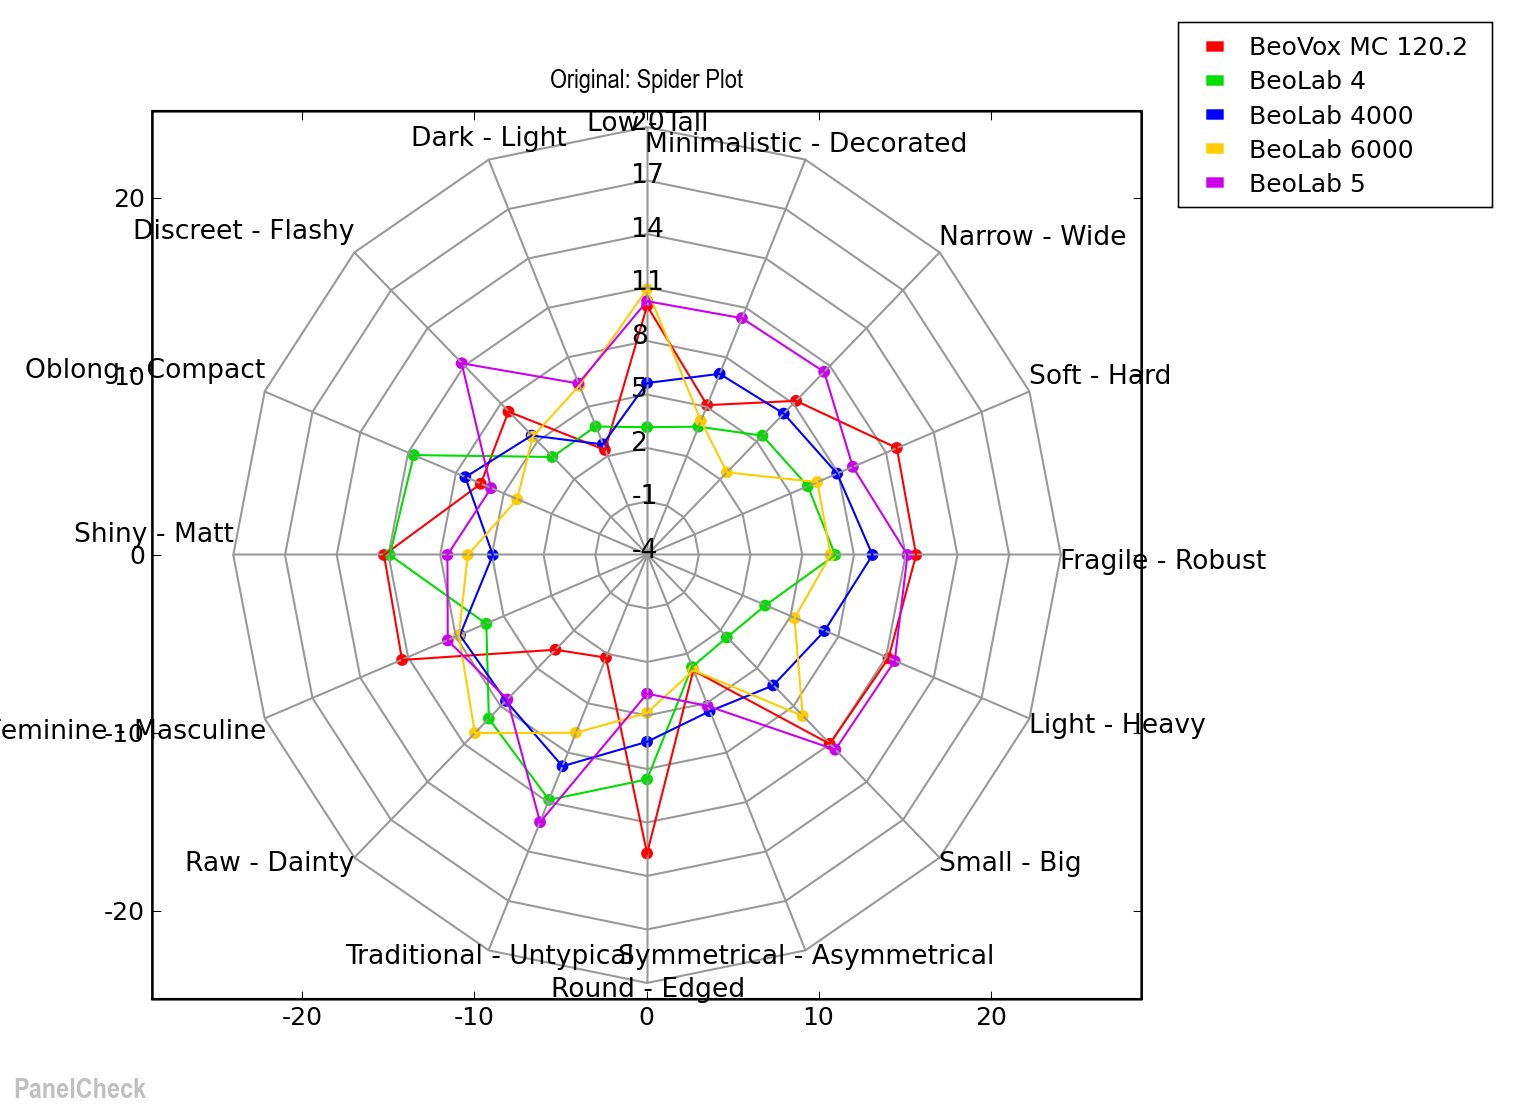
\includegraphics[width = \textwidth]{Figure/spider_plot.png}
\caption{A spider plot of the subjects' preference of the five different speakers according to each attribute.}
\label{fig:spider_plot}
\end{figure}
\newpage
%
\subsection*{Possible Correlation}
The spider plot in \autoref{fig:spider_plot} also paints an overall picture of which attributes might correlate though they are not arranged according to correlation. The plot can also get a bit confusing when multiple points are arranged close or on top of each other as previously stated. Luckily \textit{PanelCheck} contains a \textit{PCA Correlation loadings plot} which presumably arranges attributes with higher correlation close to one another. The plot is shown on \autoref{fig:pca}.
%
\begin{figure}[H]
\centering
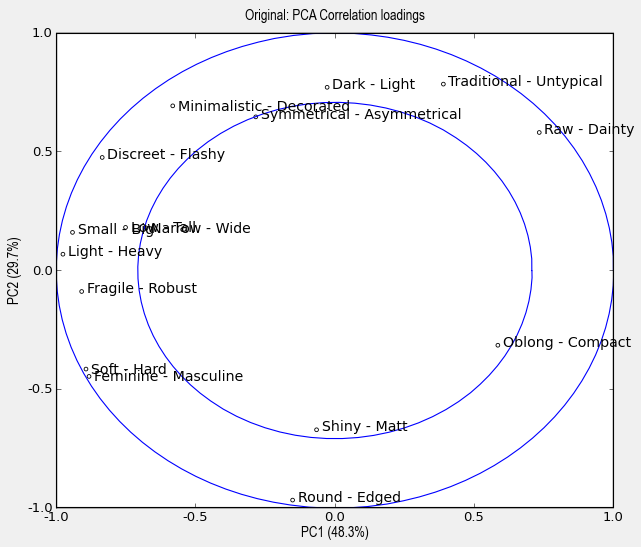
\includegraphics[width = \textwidth]{Figure/PCA_correlations.png}
\caption{A plot containing the PCA Correlation loadings. It becomes clearer which attributes correlates e.g. "Small - Big" and "Light - Heavy".}
\label{fig:pca}
\end{figure}
\noindent
%
In this PCA Correlation loadings plot a group appears to the left containing: \textit{Light - Heavy}, \textit{Small - Big}, \textit{Low - Tall}, \textit{Narrow - Wide}, and \textit{Fragile - Robust}. This means that there seems to exist a correlation with these attributes. The group makes sense from an objective point of view where all attributes relates to size except \textit{Fragile - Robust}. However small, narrow, light, etc. might often be experienced to be fragile. The same goes for robust and being big etc. Another clear group is \textit{Soft - Hard} and \textit{Feminine - Masculine}. It could be investigated further if these correlations are strong enough to stand alone meaning, perhaps they mean the same to the assessors and the number of word pairs might be reduced without losing much resolution in the data.